
\FloatBarrier
\subsection{Система Лоренца} % _LOR_

\LinkRef{
  lor: ASAU-22, 23, 24, 25, 26. APIR-2012. CSIT-2015. ISDMCI-2014, ISDMCI-2015.
  ITMM-2012, ITMM-2014, ITMM-2015, DSMP-2016
}

В качестве первой идентифицируемой хаотической системы рассмотрим
систему Лоренса, динамика которой описывается системой уравнений~[??]:

\begin{equation}
\begin{cases}
  \dot{x} = \sigma (y-x ) , \\
  \dot{y} = x (r-z) - y , \\
  \dot{z} = x y - b z .
\end{cases}
\label{atu:eq:lor}
\end{equation}

Наиболее ценным с точки зрения идентификации является параметр
$r$, определяющий как энергетическое состояние системы,
так и вид динамики системы.
Для определённости зададим остальные параметры следующим образом:
$b = 2.6666667$, $\sigma = 10$.

Критерий
$\overline{x^2}$


% Идентифицируемый параметр:
% $r \in [ 5; 100 ] $.
%
% Остальные параметры:
% $b = 2.66667$, $\sigma = 10$.

\begin{figure}[h!]
\begin{center}
  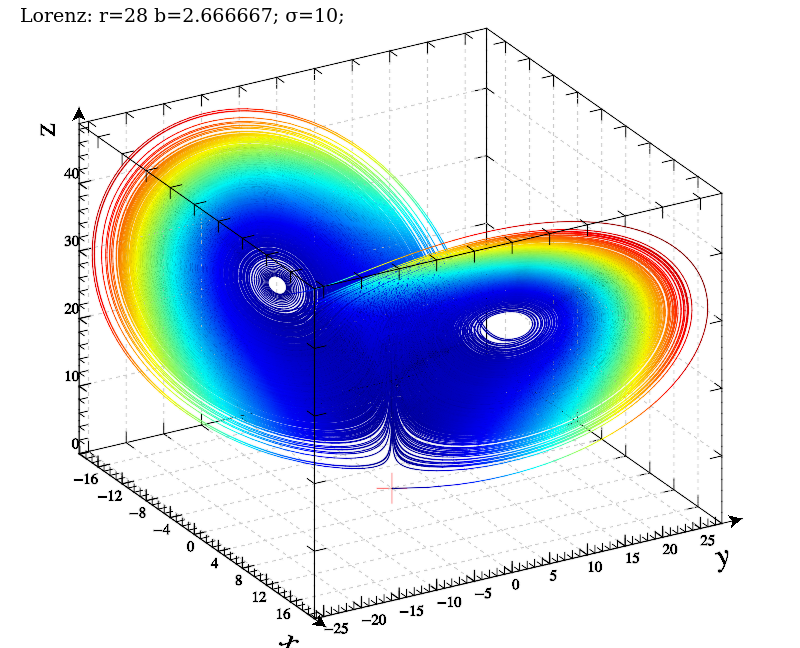
\includegraphics[width=0.45\textwidth]{p/cha/lor/lor0-p_xyz_r=28.png}
  \hfill
  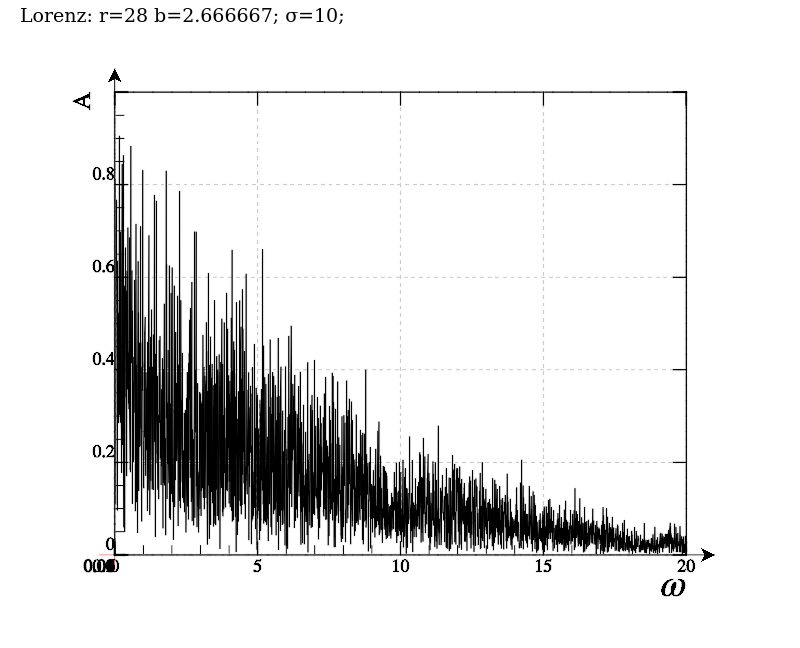
\includegraphics[width=0.45\textwidth]{p/cha/lor/lor0_fft-p_f_r=28.png}
\end{center}
\caption{Аттрактор и спектр системы Лоренца (\ref{atu:eq:lor}) в хаотическом режиме}
\label{atu:f:lor_attractor_phase_chaos}
\end{figure}

\begin{figure}[h!]
  \centerline{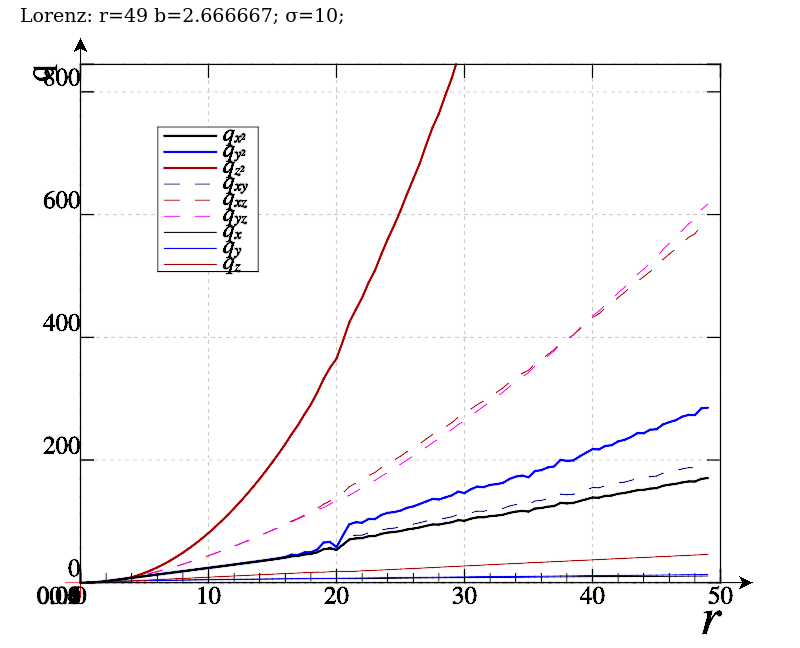
\includegraphics[width=0.7\textwidth]{p/cha/lor/lor_q-p_r.png} }
  \caption{Рассматриваемые критерии для системы Лоренца}
  \label{atu:f:lor_q}
\end{figure}

\begin{figure}[h!]
  \centerline{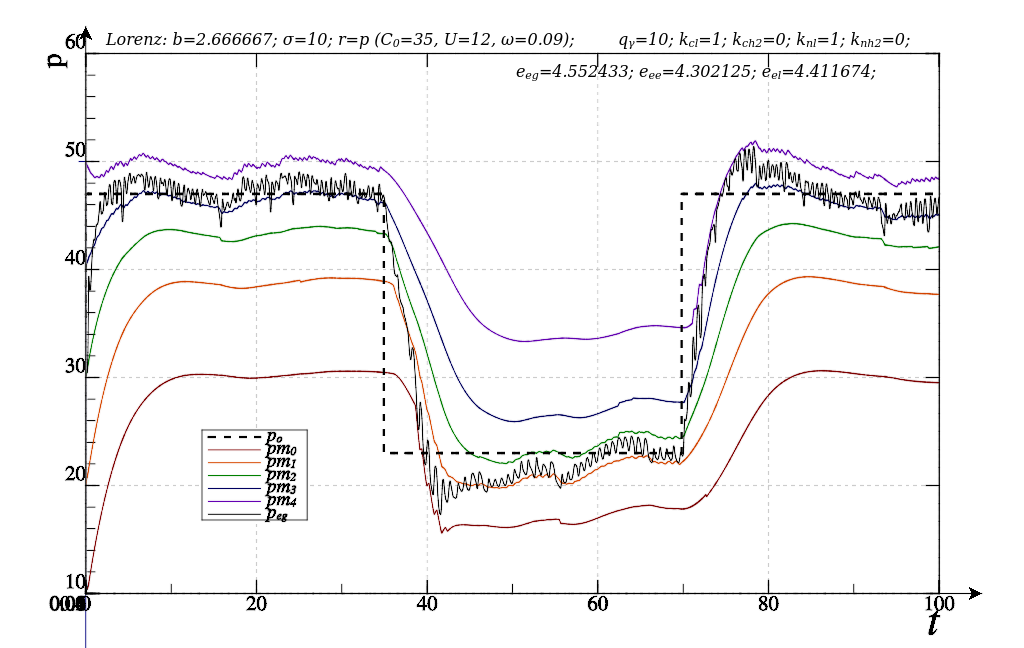
\includegraphics[width=0.7\textwidth]{p/cha/lor/lor_m5pf-pl_n_sign.png} }
  \caption{Процесс идентификации параметра ``$r$'' системы Лоренца}
  \label{atu:f:lor_id_mp5_sign}
\end{figure}

\[
  r_o(t) = p_o(t) = p_0 +  U_{p} \sign \sin( \omega_{p} t ),
\]


\begin{figure}[h!]
  \centerline{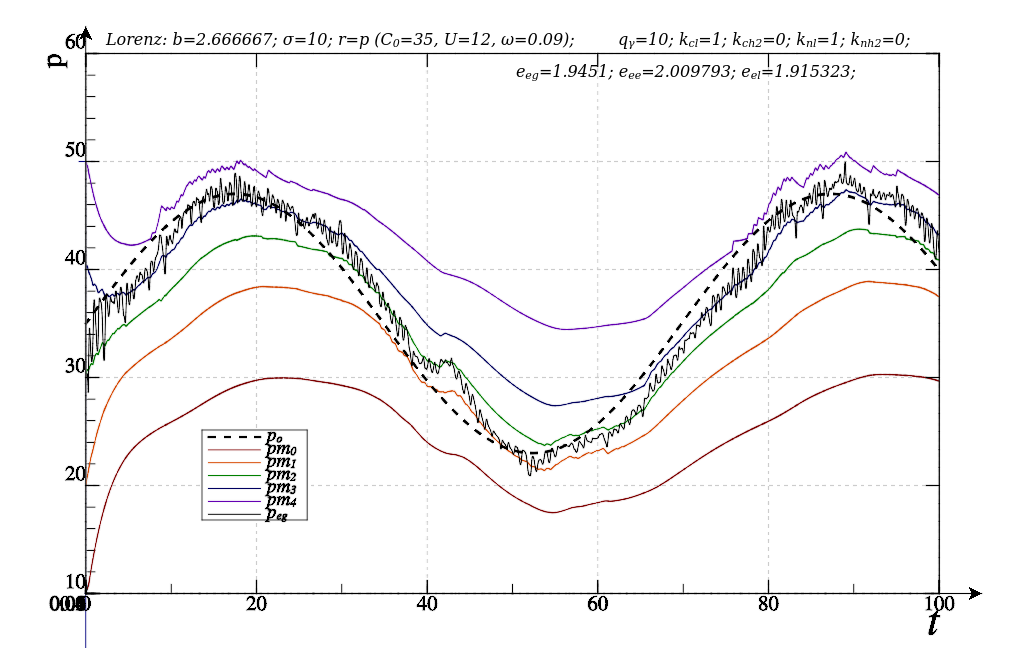
\includegraphics[width=0.7\textwidth]{p/cha/lor/lor_m5pf-pl_n_sin.png} }
  \caption{Процесс идентификации параметра ``$r$'' системы Лоренца}
  \label{atu:f:lor_id_mp5_sin}
\end{figure}

\[
  r_o(t) = p_o(t) = p_0 +  U_{p} \sin( \omega_{p} t ),
\]


